\section{Corrente. Energia potencial elétrica}

\frame{
	\frametitle{Eletrostática x Eletrodinâmica}
	\begin{block}{Eletrostática}
		\begin{itemize}
			\item Física das cargas elétricas estacionárias (em repouso).
		\end{itemize}
	\end{block}

	\begin{block}{Eletrodinâmica}
		\begin{itemize}
			\item Física das cargas elétricas em movimento.
		\end{itemize}
	\end{block}
}

\frame{
	\frametitle{Corrente Elétrica}
	\centerline{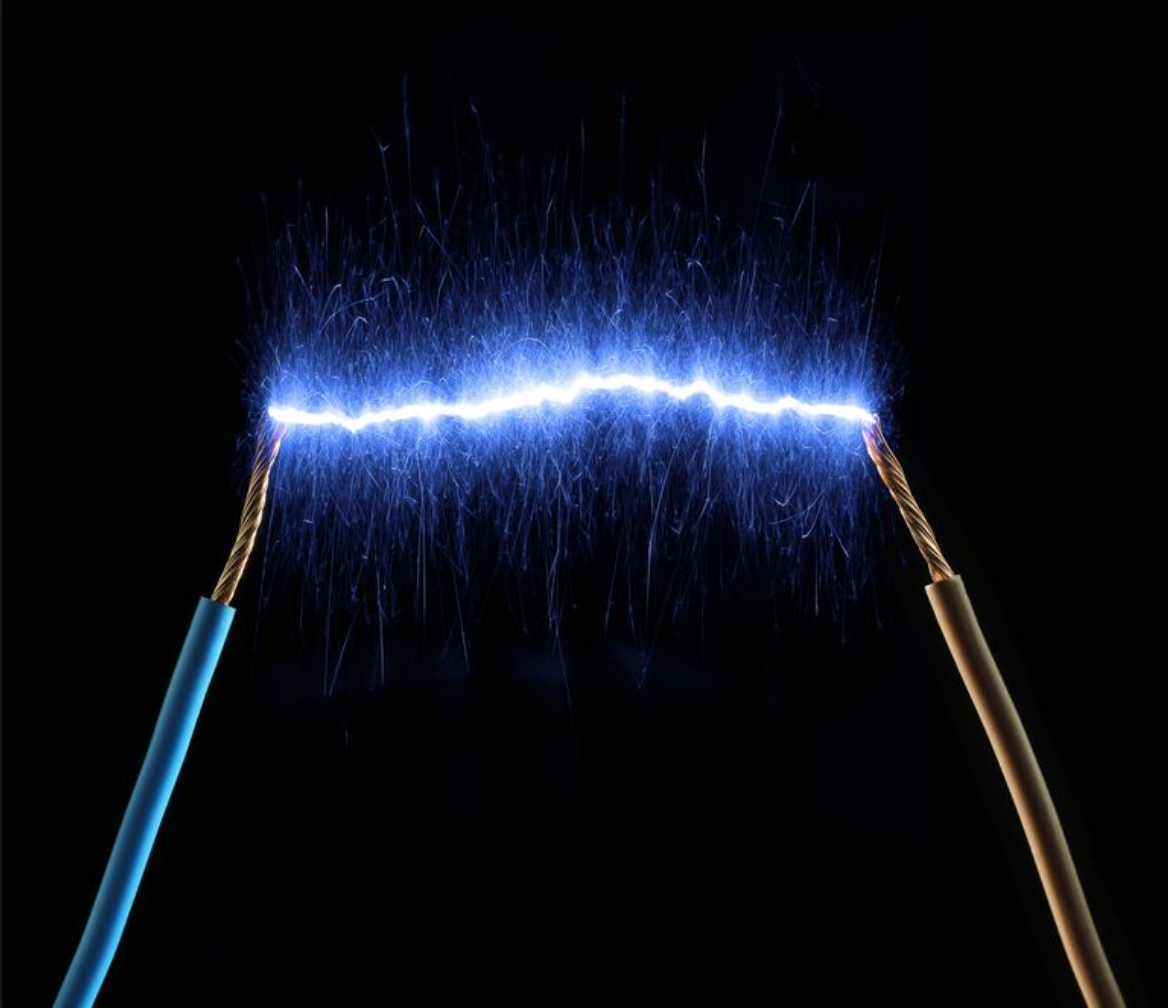
\includegraphics[width=0.7\linewidth]{Figuras/Ch11/corrente.PNG}}
}

\frame{
	\frametitle{Exemplos de aplicações}
	\begin{block}{Áreas}
		\begin{itemize}
			\item Meteorologistas: relâmpagos
			\item Bioengenharia: corrente nervosa
			\item Engenheiros eletricistas: energia elétrica
			\item Engenheiros espaciais: partículas carregadas
		\end{itemize}
	\end{block}
}



\frame{
	\frametitle{Definição}
	\begin{block}{Definição informal}
		\begin{itemize}
			\item Corrente elétrica pode ser definida como o movimento de partículas carregadas.
		\end{itemize}
	\end{block}

	\centerline{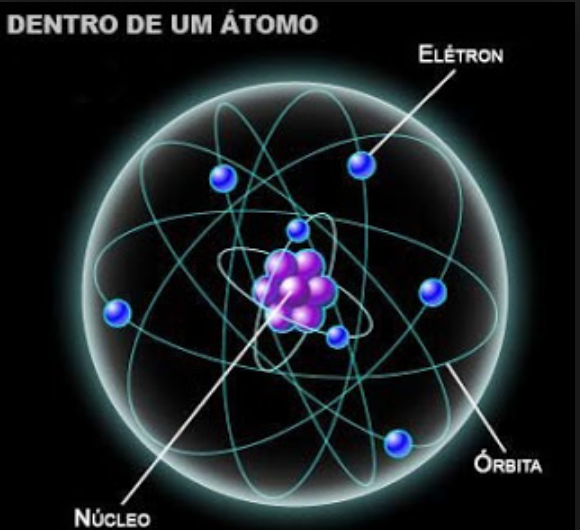
\includegraphics[width=0.5\linewidth]{Figuras/Ch11/atomo.PNG}}
}

\frame{
	\frametitle{Quem veio primeiro: o ovo ou a galinha?}
	\centerline{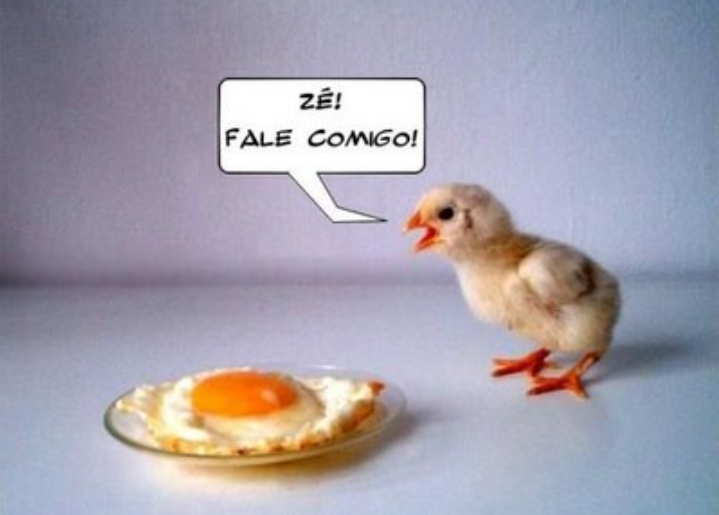
\includegraphics[width=0.9\linewidth]{Figuras/Ch11/ovo.PNG}}
}

\frame{
	\frametitle{Movimento ordenado e desordenado}
	\begin{block}{}
			\begin{itemize}
			\item Naturalmente os elétrons se encontram de maneira desordenada.
			\item O fluxo líquido em qualquer direção específica é \textit{zero}.
		\end{itemize}
	\end{block}

	\bigskip
	
	\centerline{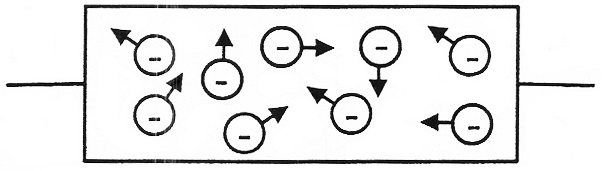
\includegraphics[width=0.9\linewidth]{Figuras/Ch11/desordenado.jpg}}
}

\frame{
	\frametitle{Movimento ordenado e desordenado}
	\begin{block}{}
		\begin{itemize}
			\item Para que esse fluxo de elétrons trabalhe é preciso uma direção - bateria no circuito.
			\item Produção de campo elétrico no interior do fio - movimento de cargas elétricas.
		\end{itemize}
	\end{block}

	\bigskip

	\centerline{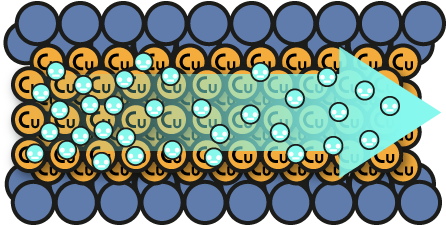
\includegraphics[width=0.7\linewidth]{Figuras/Ch11/movElet.png}}
}

\frame{
	\frametitle{Quem veio primeiro: o ovo ou a galinha?}
	\centerline{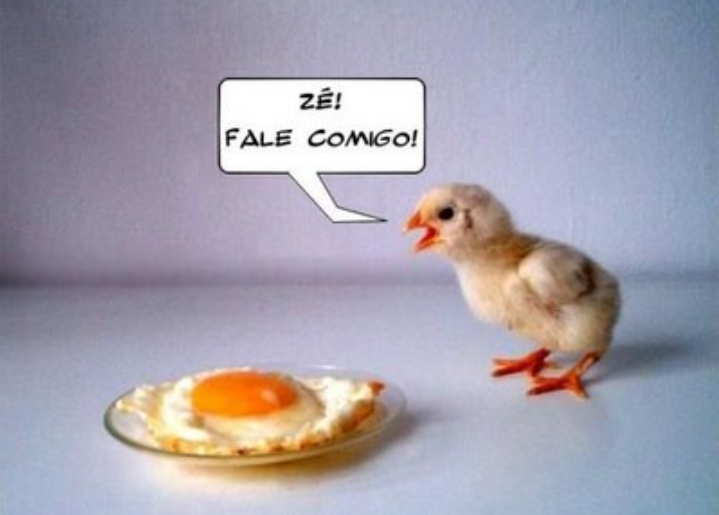
\includegraphics[width=0.6\linewidth]{Figuras/Ch11/ovo.PNG}}
	\begin{block}{Desse modo...}
		\begin{itemize}
			\item A tensão aplicada é o mecanismo de partida; a corrente é uma reação à tensão aplicada.
		\end{itemize}
	\end{block}
}

\subsection{}
\frame{
	\frametitle{Definição}
	\begin{block}{Definição formal}
		\begin{itemize}
			\item Corrente elétrica pode ser definida como o movimento \textbf{ordenado} de cargas elétricas.
		\end{itemize}
	\end{block}
}

\subsection{Unidade de medida}
\frame{
	\frametitle{André Marie Ampère}
	\centerline{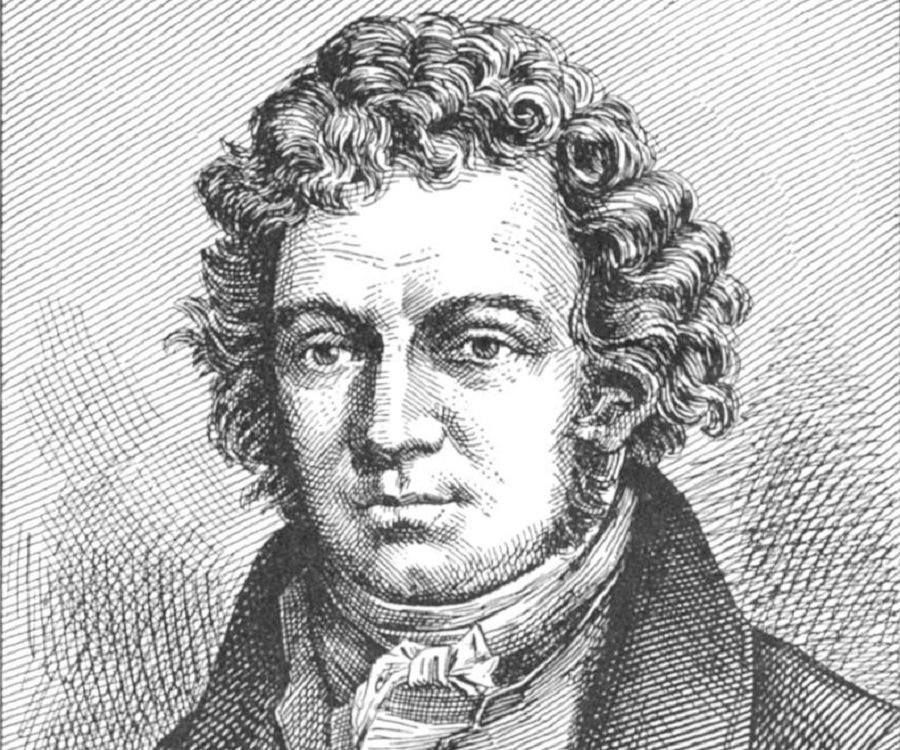
\includegraphics[width=0.4\linewidth]{Figuras/Ch11/ampere.png}}
	\begin{block}{Intensidade da Corrente Elétrica}
		$$\boxed{I = \frac{Q}{t}} \qquad [\si{\ampere}]$$
	\end{block}
}

\subsection{Sentido da corrente}
\frame{
	\frametitle{Sentido convencional ou real}
	\begin{block}{Convenção}
		\begin{itemize}
			\item Sentido real: movimentação ordenada de elétrons (cargas negativas).
			\item Sentido convencional: por razões históricas a seta da corrente é desenhada no sentido em que portadores de carga positivos se movam.
		\end{itemize}
	\end{block}

	\bigskip
	
	\centerline{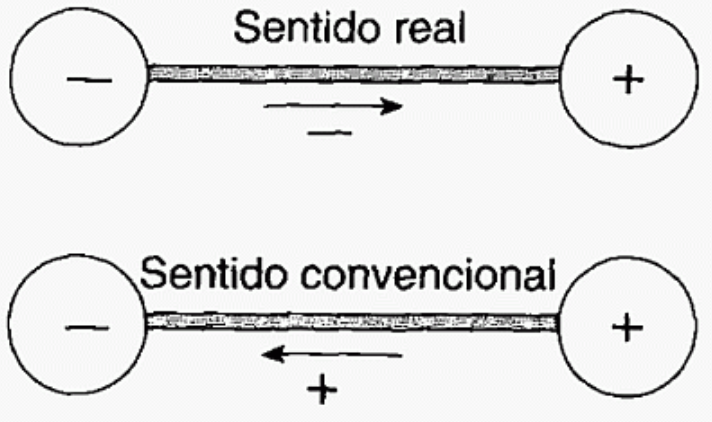
\includegraphics[width=0.55\linewidth]{Figuras/Ch11/real.PNG}}
}

\subsection{}
\frame{
	\frametitle{Especificação Ampère-Hora}
	\begin{block}{Vida útil da bateria}
		\begin{itemize}
			\item Utilizado para determinar o tempo de duração de uma bateria.
		\end{itemize}
		
		\medskip
	
		$$\text{vida útil da bateria} = \frac{\text{capacidade da bateria}}{\text{consumo do dispositivo}}$$
	\end{block}
	
	\medskip

	\centerline{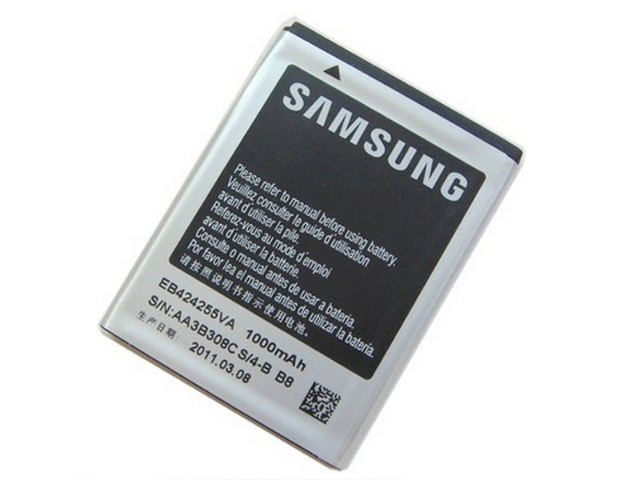
\includegraphics[width=0.4\linewidth]{Figuras/Ch11/bateria.jpg}}
}

\subsection{Potencial Elétrico}
\frame{
	\frametitle{Alessandro Antonio Volta}
	\centerline{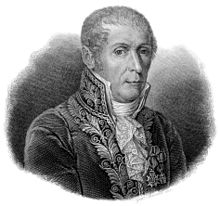
\includegraphics[width=0.4\linewidth]{Figuras/Ch11/volts.png}}
	\begin{block}{Tensão Elétrica}
		\begin{itemize}
			\item Tensão (ou diferença de potencial) é a energia necessária para deslocar
			      uma carga unitária através de um elemento.
		\end{itemize}
		$$\boxed{U = \frac{\tau}{\Delta Q}} \qquad [\si{\volt}]$$
	\end{block}
}

\section*{Exercícios}

\frame{
	\frametitle{Exercícios}
	\begin{block}{}
		01. Por quanto tempo uma bateria de transistor \SI{9}{\volt} com uma especificação ampère-hora de \SI{520}{\milli\ampere\hour} vai fornecer uma corrente de \SI{20}{\milli\ampere}?

		\vspace{1cm}

		02. Por uma seção transversal de um condutor metálico passa uma carga elétrica total $\Delta q = \SI{4}{\milli\coulomb} $ no intervalo de tempo $\Delta t = \SI{20}{\second}$. Determine a intensidade da corrente e o número de elétrons que passam em um segundo.

	\end{block}
}

\section*{Referências}

\frame{
	\frametitle{Referências e Exercícios Complementares}
	\begin{itemize}
		\item Física, Ciência e Tecnologia – Vol 3. PENTEADO, Paulo César M; TORRES, Carlos Magno A. Ed. Moderna (2006)
	\end{itemize}
	%\centering{\alert{Página 36 - \textbf{1.6.1 até 1.6.5, 1.6.17 até 1.6.19}}} \\
	\centering{\alert{Lista de exercícios 11}}
}